% 导言区 -------------------------------------------------
\documentclass[aspectratio=169,t,xcolor=table,10pt]{ctexbeamer}
\usetheme{CHD}

% 宏包 **************************************
\usepackage[utf8]{inputenc}
\usepackage{ctex} % 中文宏包
\usepackage{xcolor} % 颜色宏包
\usepackage{tcolorbox} % 颜色盒子
\usepackage{booktabs} % 三线表
\usepackage{subcaption} % 子图和标题
\usepackage{float} % 修改浮动体宏包
\usepackage{hyperref} % 超链接
\usepackage{tikz} % 绘图宏包
\usepackage{float} % 浮动体[H]参数即为禁止浮动
\usepackage{graphics} % 图像宏包
\usepackage{subcaption} % 子图和标题
\usepackage{wallpaper}
\usepackage{background}
\setbeamercovered{transparent}

% 数学类宏包 **************************************
\usepackage{amsmath} % AMS 数学宏包
\usepackage{amssymb} % AMS 符号宏包
\usepackage{mathrsfs} % 花体符号宏包 \mathscr{}
\usepackage{amsthm} % 数学证明宏包
\usepackage{accents} % 重音



% 作者信息 -------------------------------------------
\title{\Huge{基于机器视觉的铣刀状态在机监测方法研究}}
%\subtitle{ }
\author{\large{小组成员:XXX \ XXX \ XXX \ XXX \ XXX}}

\institute{\large{仪器科学与光电工程学院 }}
\date{\today}


% 模板设置 -------------------------------------------
\setPrimaryColor{CHDred}
\setLogos{lib/CHDlogo/CHDname-white.pdf}{lib/CHDlogo/infw2.pdf}
\usefonttheme{serif} % 修改公式字体为衬线字体
\setbeamertemplate{caption}[numbered] % 开启 caption 计数
\numberwithin{equation}{section} % 公式开启 subsection 计数

% 自定义命令 ------------------------------------------
\newcommand{\bbr}{\mathbb{R}}
\newcommand{\norm}[1]{\left||{#1}\right||}
\newcommand{\ubar}[1]{\underaccent{\bar}{#1}}

% 超链接形式修改
% \definecolor{linkcol}{RGB}{201,55,86} % ref 类的颜色
\definecolor{urlcol}{RGB}{84,150,136} % url 类的颜色
\definecolor{citecol}{RGB}{75,92,196} % cite 类的颜色
\hypersetup{
	colorlinks=true, % 颜色超链接,不用框
	linkcolor=CHDred, % ref 类的颜色
	urlcolor=urlcol, % url 类的颜色
	citecolor=citecol, % cite 类的颜色
	pdfstartview=Fit,
	breaklinks=true,
	% citecolor=black,
	% filecolor=black,
}

% 正文 -------------------------------------------
\begin{document}
	
	% #################### 封面页 ####################
	\frame[noframenumbering]{\titlepage}
	
	
	% #################### 目录页 ####################
	\setLayout{horizontal} % 当前 frame 的布局,可选择:'horizontal','vertical', 'blank, 'mainpoint', 'titlepage'
	\begin{frame}
		\frametitle{目录 Contents}
		\begin{center}
			\large{
				\tableofcontents[hideallsubsections]
			}
		\end{center}
	\end{frame}


	% #################### section1 ####################
	% 每个 section 开始之前,生成当前目录
	\setLayout{mainpoint} % 当前 frame 的布局,可选择:'horizontal','vertical', 'blank, 'mainpoint', 'titlepage'
	\section{课题介绍}
	\begin{frame}
		\frametitle{课题介绍}
	\end{frame}

	\setLayout{horizontal} % 当前 frame 的布局,可选择:'horizontal','vertical', 'blank, 'mainpoint', 'titlepage'
	\begin{frame}
		\begin{block}{问题概述与脉络分析}
			\qquad 刀具作为数控机床切削过程中的直接执行者,其磨损状态是影响被加工工件的表面质量和尺寸精度的重要因素。因此需要建立一个在不停机的动态情况下的刀具监测系统。
			\begin{itemize}[<+->]
				\item 搭建硬件监测系统并且对硬件进行选型,并且寻找相机部署距离和曝光时间的最优解。
				\item 确定动态图像序列中刀具磨损图像的起始帧和终止帧。
				\item 实现磨损区域的精确分割和测量。
			\end{itemize}
		\end{block}
	\end{frame}
	

	% #################### section2 ####################
	\section{系统设计与部署}
	% 每个 section 开始之前,生成当前目录
	\setLayout{mainpoint} % 当前 frame 的布局,可选择:'horizontal','vertical', 'blank, 'mainpoint', 'titlepage'
	\begin{frame}
		\frametitle{系统设计与部署}
	\end{frame}
	
	\setLayout{vertical} % 当前 frame 的布局,可选择:'horizontal','vertical', 'blank, 'mainpoint', 'titlepage'
	\subsection{机器视觉监测系统设计}
	\begin{frame}
		\frametitle{机器视觉监测系统设计}
		\begin{block}{系统图}
			\qquad 基于机器视觉的铣刀状态在机监测系统如下图所示:
			\begin{figure}[H]
				\centering
				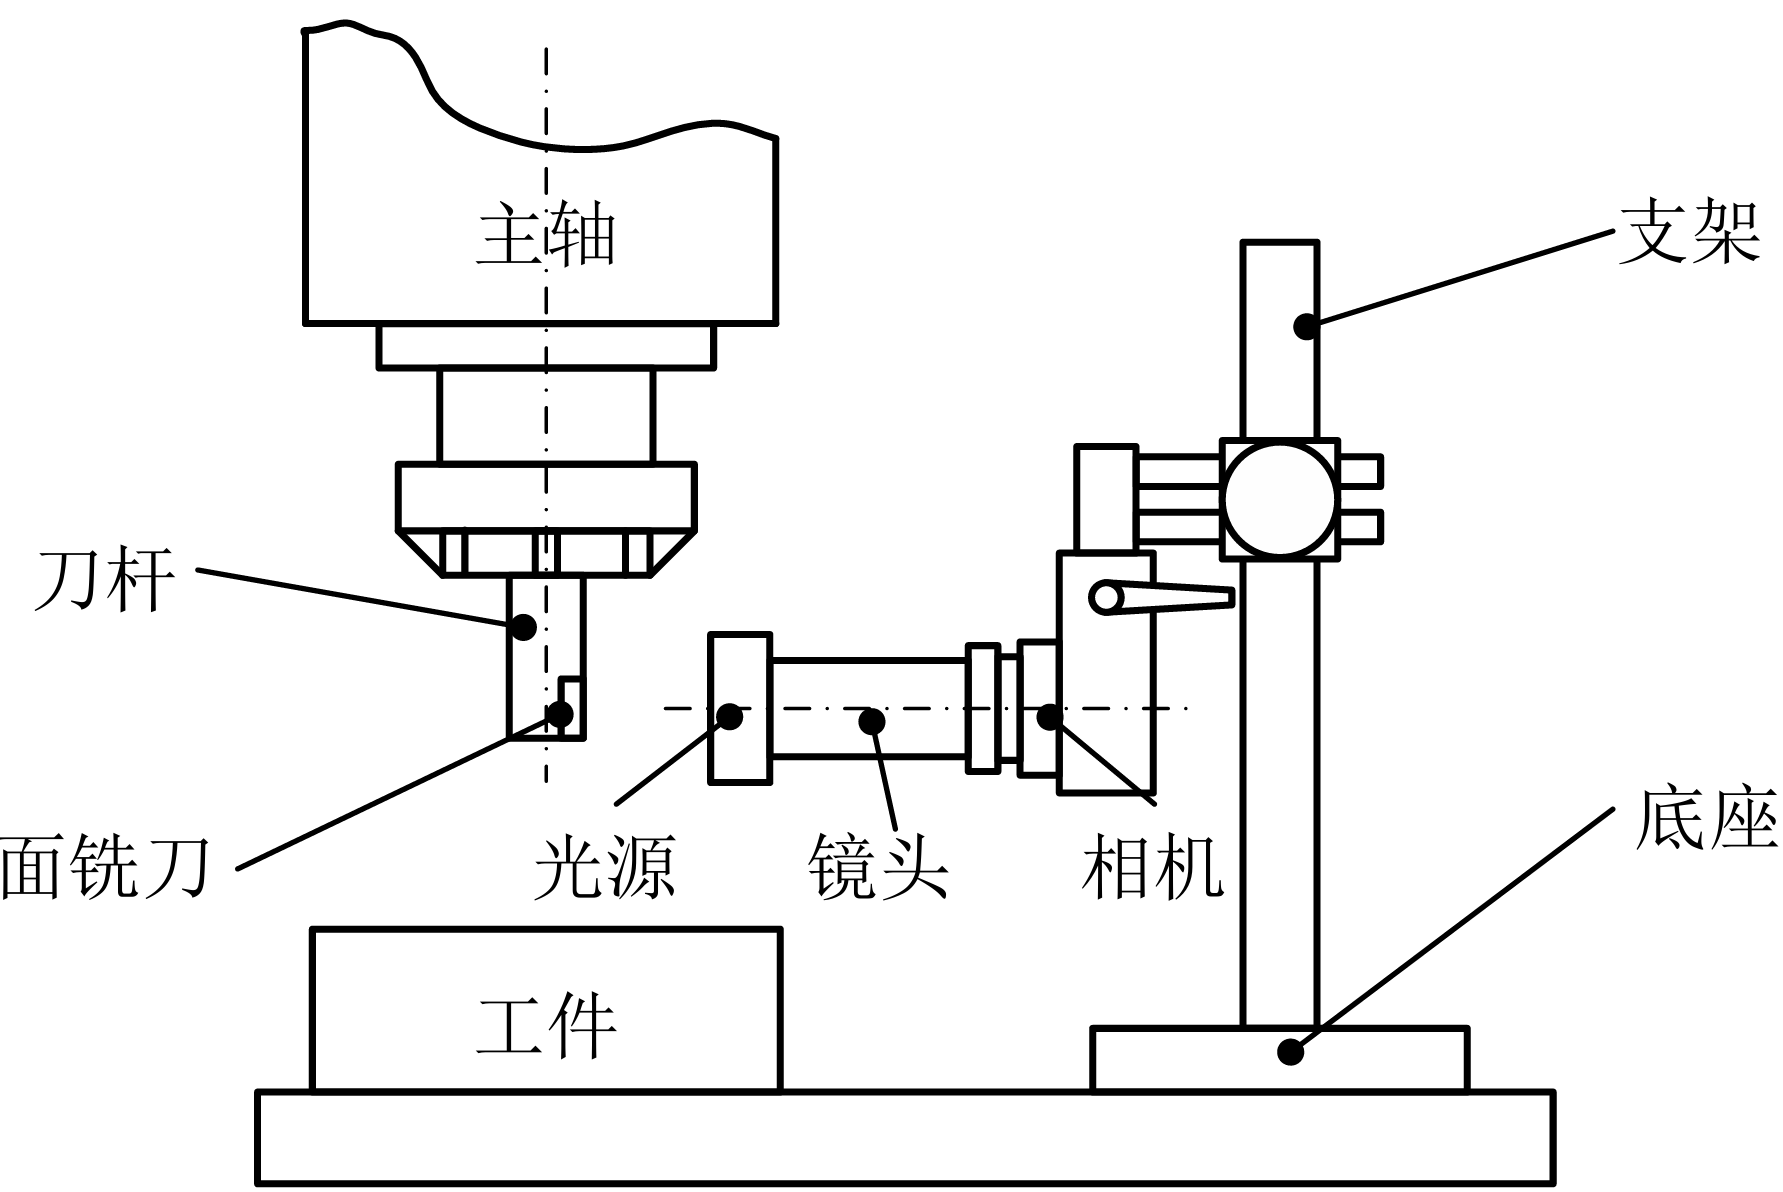
\includegraphics[width=0.5\linewidth]{Figure/System}
				\caption{机器视觉监测系统示意图}
			\end{figure}
		\end{block}
	\end{frame}

	\begin{frame}[squeeze]
		\begin{block}{相机}
			\qquad 在给定视场和检测精度,相机的分辨率计算为
			\begin{equation}
				R_a\ge R_i = \frac{FOV}{A_c}
				\label{fenbianlv}
			\end{equation}
			\eqref{fenbianlv} 中,$FOV$ 表示目标的宽度和高度($\mathrm{mm}$);$A_c$ 表示通过机器视觉系统进行目标检测所需的精度($\mathrm{mm}$);$R_i$ 表示理想计算条件下工业相机采集图像的像素总数(pixel);$R_a$ 表示实际工业相机采集图像的像素总数(pixel),由工业相机分辨率所决定。
			
			\qquad 在加工过程中,刀具固定在刀杆上并随之旋转。因此,相机的宽视场由刀杆参数决定
			\begin{equation}
				FOV = \sin(\frac{90}{n})R_h
				\label{FOV}
			\end{equation}
			式中,$n$ 表示固定在刀杆上的刀具数量;$R_h$ 表示刀杆的直径($\mathrm{mm}$)。 根据国内外研究,$A_c=50\mathrm{\mu m}$ 时达到有效的刀具磨损监测效果。
			
			\qquad 相机需要具有较高的帧率以满足刀具磨损状态在线和实时检测的要求。为了保证拍摄图像的清晰,相机的帧率和主轴转速的关系如式
			\begin{equation}
				\frac{n\times\pi R_h}{60}<\frac{FOV}{\sigma}R_f
				\label{zhenlv}
			\end{equation}
		\end{block}
	\end{frame}
	
	\begin{frame}[squeeze]
		\begin{block}{相机}
			\qquad 综合考虑以上因素,本章选择德国 Basler 公司型号为 acA2040-90um 的 CMOS 相机,该相机的如下图所示:
			\begin{figure}[H]
				\centering
				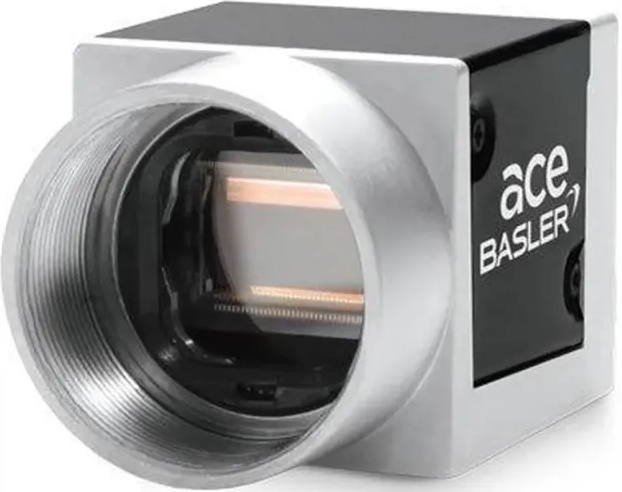
\includegraphics[width=0.5\linewidth]{Figure/Basler}
				\caption{CMOS 相机实物}
			\end{figure}
		\end{block}
	\end{frame}
	
	\begin{frame}[squeeze]
		\begin{block}{相机}
			\qquad 参数如下表所示:
			\begin{table}[H]
				\centering
				\caption{德国 Basler 公司型号为 acA2040-90um 相机的主要参数}
				\begin{tabular}{cc|cc}
					\toprule[1.5pt]
					参数内容 & 参数值 & 参数内容 & 参数值 \\
					\midrule[0.75pt]
					感光芯片供应商 & ams & 黑白/彩色 & 黑白 \\
					快门类型 & 全局快门 & 动态范围(dB) & 58.7 \\
					芯片尺寸(英寸) & 1 & 信噪比(dB)& 40.8 \\
					感光芯片类型 & CMOS & 数据接口 & USB 3.0  \\
					感光芯片尺寸($\mathrm{mm}$)& 11.3×11.3 & 像素位深(bits)& 10,12 \\
					水平/垂直分辨率(pixel) & 2048×2048 & 外形尺寸($\mathrm{mm}$) & 29.3×29×29 \\ 
					水平/垂直像素尺寸(μm) & 5.5×5.5 & 功耗(W) & 3.2 \\
					帧率(fps) & 90 & 镜头接口 &  C-mount  \\
					\bottomrule[1.5pt]
				\end{tabular}
				\label{CMOScanshu}
			\end{table}
		\end{block}
	\end{frame}
	
	\begin{frame}[squeeze]
		\begin{block}{镜头}
			\qquad 在对比不同类型的镜头之后,双远心镜头采用了一种独特的光路设计,且具有无透视误差、近乎零失真度、高分辨率、放大率一致和较长景深的优点。根据表 \ref{CMOScanshu} 的参数以及 \eqref{fenbianlv}\eqref{FOV}\eqref{zhenlv} 维视智造公司型号为 BT-2307 的双远心镜头如图所示:
			\begin{figure}[H]
				\centering
				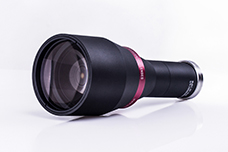
\includegraphics[width=0.5\linewidth]{Figure/BT}
				\caption{BT-2307双远心镜头实物图 }
			\end{figure}
		\end{block}
	\end{frame}

	\begin{frame}[squeeze]
		\begin{block}{镜头}
			\qquad 参数如下表所示:
			\begin{table}[H]
				\centering
				\caption{BT-2307 双远心镜头参数}
				\begin{tabular}{c|c}
					\toprule[1.5pt]
					参数内容 & 参数值 \\
					\midrule[0.75pt]
					放大倍率  & 1.333 \\
					视场宽高(mm)或 CCD 靶面尺寸 & 2/3'' $6.6\times5.0$ \\
					光圈 & 11  \\
					远心度 & $<0.08^{\circ}$  \\
					工作距离(mm) & $61.2\pm3\%$  \\
					景深(mm) & 0.5 \\ 
					畸变(\%) &  <0.05  \\
					\bottomrule[1.5pt]
				\end{tabular}
				\label{BTcanshu}
			\end{table}
			\qquad 综上所述,在选定相机型号和镜头型号的基础上,宽视场的机器视觉监测系统成像的参数如下:相机视野大小为 $8.4\mathrm{mm}\times8.4\mathrm{mm}$,图像分辨率为 $2048\times2048$,一个像素代表 $4.125\mathrm{\mu m}$。在加工过程中使用的面铣刀刀片型号为 Duracarb APMT1135,其厚度为 $3.5\mathrm{mm}$,搭建的机器视觉监测系统的视野范围是该厚度的 2.4 倍,满足 \eqref{fenbianlv} 和 \eqref{FOV} 宽视场的定义。
		\end{block}
	\end{frame}

	\begin{frame}[squeeze]
		\begin{block}{光源}
			\qquad 在光源设计时,需要综合考虑光源类型、布置方式以及与镜头匹配等多种因素。由于双远心镜头只接受平行光,滤除了几乎所有的漫反射光源。因此,本章选用平行光源,以满足双远心镜头对入射光类型的要求。综合分析,环形 LED 光源满足以上条件,其具有高亮度,便于安装,结构灵活的特点。本章选用维视智造 AFT-RL5428-29W 环形光源,该光源亮度可调、性能稳定、超长寿命、无阴影,常用于机器视觉和工业检测场景,如下图所示:
			\begin{figure}[H]
				\centering
				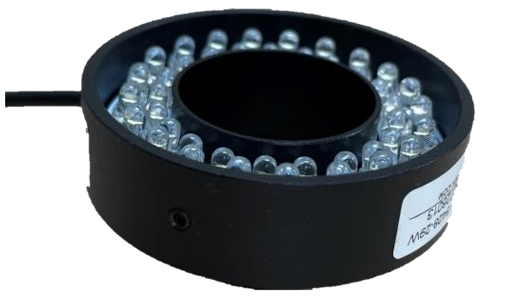
\includegraphics[width=0.5\linewidth]{Figure/AFT}
				\caption{AFT-RL5428-29W 环形光实物图}
			\end{figure}
		\end{block}
	\end{frame}

	\subsection{机器视觉监测系统部署}
	\begin{frame}
		\frametitle{机器视觉监测系统部署}
		\begin{block}{部署模型构建思路}
			\qquad 需要建立对捕获的图像的评价模型,以寻求最优的相机工作距离和曝光时间。注意,这里图像没有参考图像判断质量优劣,这是一个无参考质量评价问题,这也是一个在相机校准中的普遍问题。
		\end{block}
		\begin{block}{确定无参考图像评价函数}
			\qquad 本文选择信息熵评价函数。根据香农理论,熵值较大则表示图像信息丰富度高。因此,图像的熵可以衡量图像信息的丰富程度,其定义为
			\begin{equation}
				D_{Et} = -\sum_{i=1}^{255}P_i\log{P_i}
				\label{shanghanshu}
			\end{equation}
			\eqref{shanghanshu} 中 $D_{Et}$ 表示图像熵评价函数;$P_i$ 表示图像取灰度值为 $i$ 的概率。
		\end{block}	
	\end{frame}
	
	\begin{frame}
		\begin{block}{多项式回归模型}
			\qquad 在相机部署过程中,相机工作距离和曝光时间与评价指标之间存在某种映射关系,这里不妨假设为多项式模型。设在第 $i$ 次实验下的工作距离 $d_i$ 和曝光时间 $t_i$,对于获得的第 $i$ 张图像其评价指标为 $y_i$。不妨设 $n$ 次多项式模型为
			\begin{equation}
				f(d,t)=\sum_{k=0}^{n}\sum_{r_1+r_2=k}a_{(r_1,r_2)}d^{r_1}t^{r_2}
			\end{equation}
			则对应的优化模型表述为
			\begin{equation}
				\min_{a_{(r_1,r_2)}}\sum_{i=1}^{n}\norm{f(d_i,t_i)-y_i}_2^2
				\label{duoxiangshi}
			\end{equation}
		\end{block}
		\begin{block}{优化求解}
			\qquad 利用 Powell 优化算法即可求解 \eqref{duoxiangshi},不断改变 $n$ 的次数,重复求解。寻找合适 $n$ 值和该 $n$ 值下的最优解 $(d^*,y^*)$。
		\end{block}
	\end{frame}

	\begin{frame}
		\begin{block}{求解结果}
			\qquad 得到最优的相机部署条件为:工作距离为 $231.95219091\mathrm{mm}$,相机曝光时间为 $1307\mathrm{\mu s}$。由于机床工作台运动精度限制,相机工作距离最优选择为 $231.952\mathrm{mm}$。多项式回归模型的函数关系如下图所示:
			\begin{figure}[H]
				\centering
				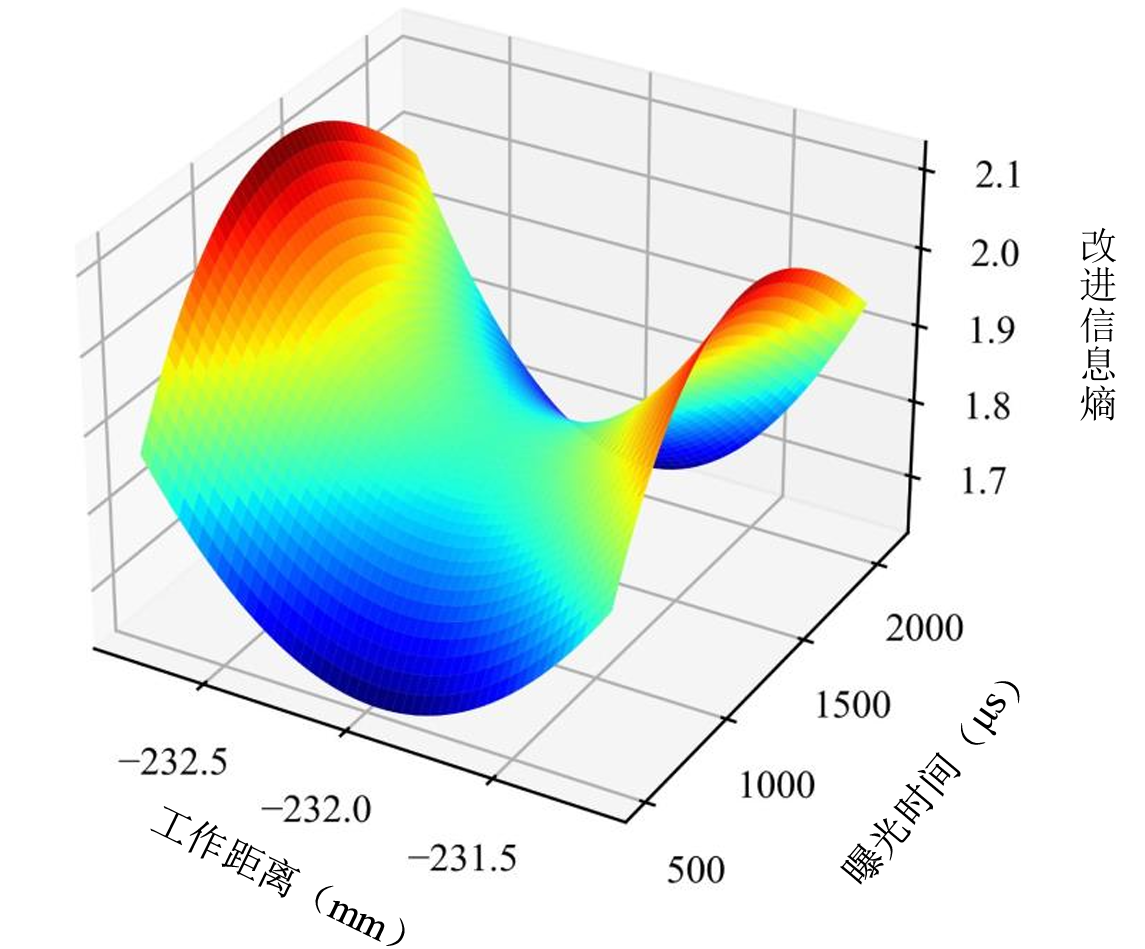
\includegraphics[width=0.5\linewidth]{Figure/Res1}
				\caption{多项式回归模型的三维图}
			\end{figure}
		\end{block}
	\end{frame}


	% #################### section3 ####################
	\section{磨损时序确定}
	% 每个 section 开始之前,生成当前目录
	\setLayout{mainpoint} % 当前 frame 的布局,可选择:'horizontal','vertical', 'blank, 'mainpoint', 'titlepage'
	\begin{frame}
		\frametitle{磨损时序确定}
	\end{frame}
	
	\setLayout{vertical} % 当前 frame 的布局,可选择:'horizontal','vertical', 'blank, 'mainpoint', 'titlepage'
	\subsection{主轴旋转下刀具磨损图像序列}
	\begin{frame}
		\frametitle{主轴旋转下刀具磨损图像序列}
		\begin{block}{刀具状态图像}
			\qquad 刀具本身是粗糙的,如果出现磨损将会表现的光滑。光源打在刀具上经过反射进入相机成像。前者相比后者的亮度将会降低。效果如下图所示:
			\begin{figure}[H]
				\centering
				\subfloat[正常刀具图像]{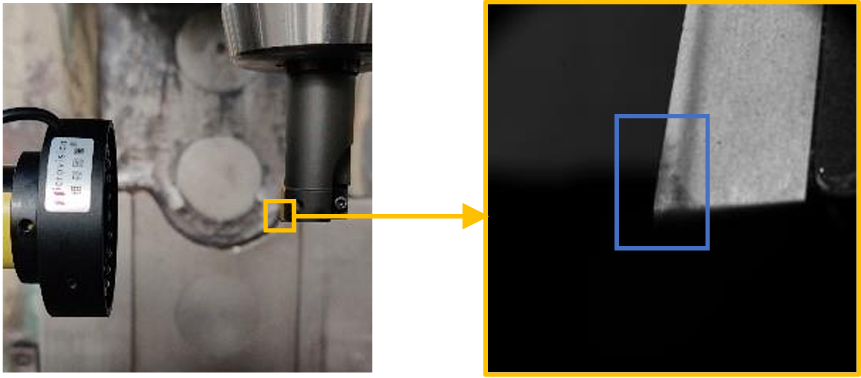
\includegraphics[width=0.4\linewidth]{Figure/daoju}}
				\hspace*{2pt}
				\subfloat[磨损刀具图像]{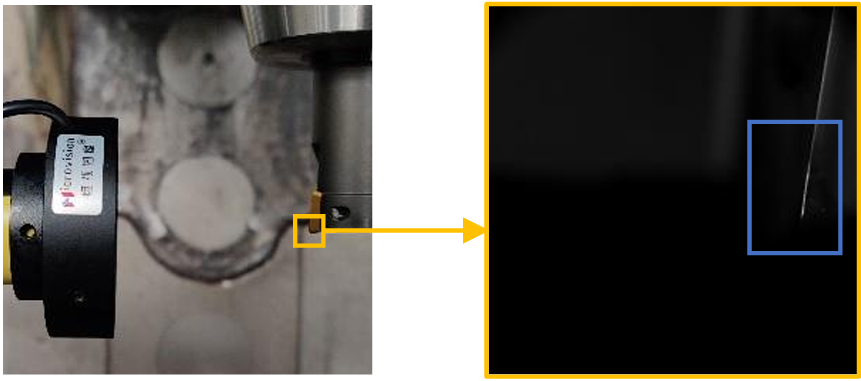
\includegraphics[width=0.4\linewidth]{Figure/daojumosun}}
			\end{figure}
		\end{block}
		\begin{block}{刀具状态图像序列(TCIS)}
			\qquad 多张连续的刀具图像序列称为刀具状态图像序列(TCIS),对于磨损刀具,其磨损区域的反射分量接近于 1。此时,刀具磨损区域特征在 TCIS 中得到增强。
		\end{block}
	\end{frame}

	\subsection{刀具磨损时序的定位}
	\begin{frame}
		\frametitle{刀具磨损时序的定位}
		\begin{block}{基于梯度直方图的图像序列初始定位}
			\qquad 对于前后两帧的图像,其梯度变化最大时,即为磨损区域的序列开始。如下图所示:
			\begin{figure}[H]
				\centering
				\subfloat[TCIS 前一帧]{
\includegraphics[width=0.3\linewidth]{Figure/qianyizhen}}
				\hspace*{48pt}
				\subfloat[TCIS 初始帧]{
\includegraphics[width=0.3\linewidth]{Figure/qishizhen}}
			\end{figure}
		\end{block}
	\end{frame}

	\begin{frame}
		\begin{block}{基于梯度直方图的图像序列初始定位}
			\qquad 定向梯度直方图是基于稠密网格中归一化的局部方向梯度直方图的计算。通过图像中局部梯度或边缘方向分布的方式以实现目标外观和形状的描述。像素点 $(x,y)$ 处的梯度大小和梯度方向为
			\begin{equation}
				\begin{cases}
					G(x,y) = \sqrt{\left[I(x+1,y)-I(x-1,y)\right]^2+\left[I(x,y+1)-I(x,y-1)\right]^2} \\
					\alpha(x,y) = \arctan\left(\dfrac{I(x,y+1)-I(x,y-1)}{I(x+1,y)-I(x-1,y)}\right)
				\end{cases}
			\end{equation}
			其中,$I(x,y)$ 表示 $(x,y)$ 处的灰度值。$G(x,y)$ 和 $\alpha(x,y)$ 表示$(x,y)$ 处的梯度和梯度方向。
			
			\qquad 当前后两帧的总 $G(x,y)$ 之差最大时,认为进入了刀具磨损的时序。
		\end{block}
	\end{frame}

	\begin{frame}
		\begin{block}{基于逻辑回归的图像序列终止定位}
			\qquad 终止帧是指在连续图像序列中高对比度刀具磨损区域最后出现的图像帧如下图所示:
			\begin{figure}[H]
				\centering
				\subfloat[TCIS 终止帧]{
\includegraphics[width=0.3\linewidth]{Figure/zhongzhizhen}}
				\hspace*{48pt}
				\subfloat[TCIS 后一帧]{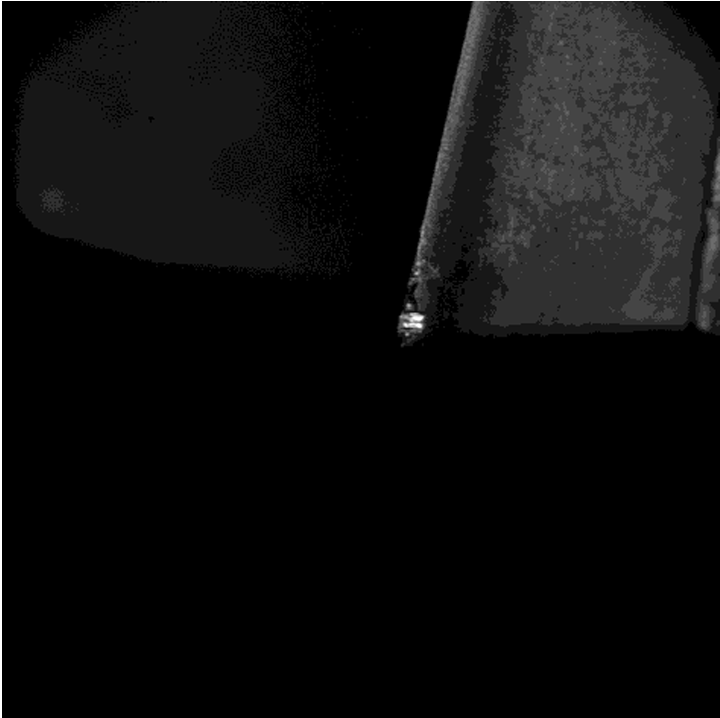
\includegraphics[width=0.3\linewidth]{Figure/houyizhen}}
			\end{figure}
			将每张捕获的图像 $\boldsymbol{C}_i$ 分解为全局图像 $\boldsymbol{G}_i$ 和阈值图像 $\boldsymbol{T}_i$ 和 $\boldsymbol{T}_i$ 各自对应的平均灰度、灰度方差、平均梯度和梯度方差,共 8 个指标作为图像 $\boldsymbol{C}_i$ 的特征向量。
			
			\qquad 构建二分类的逻辑回归模型,利用多次捕获的图像和人工标签,即可完成该模型的训练求解。最后在实践中,预测概率大于 0.5 即可认为到达终止帧。
		\end{block}
	\end{frame}


	% #################### section4 ####################
	\section{磨损精确分割测量}
	% 每个 section 开始之前,生成当前目录
	\setLayout{mainpoint} % 当前 frame 的布局,可选择:'horizontal','vertical', 'blank, 'mainpoint', 'titlepage'
	\begin{frame}
		\frametitle{磨损精确分割测量}
	\end{frame}
	
	\setLayout{vertical} % 当前 frame 的布局,可选择:'horizontal','vertical', 'blank, 'mainpoint', 'titlepage'
	\subsection{刀面磨损分割与测量}
	\begin{frame}
		\frametitle{刀面磨损分割与测量}
		\begin{block}{GrabCut 分割算法(GMM模型 \& 最小割最大流模型)}
			\qquad GrabCut 模型的图像分割的步骤如下图所示:
			\begin{figure}[H]
				\centering
				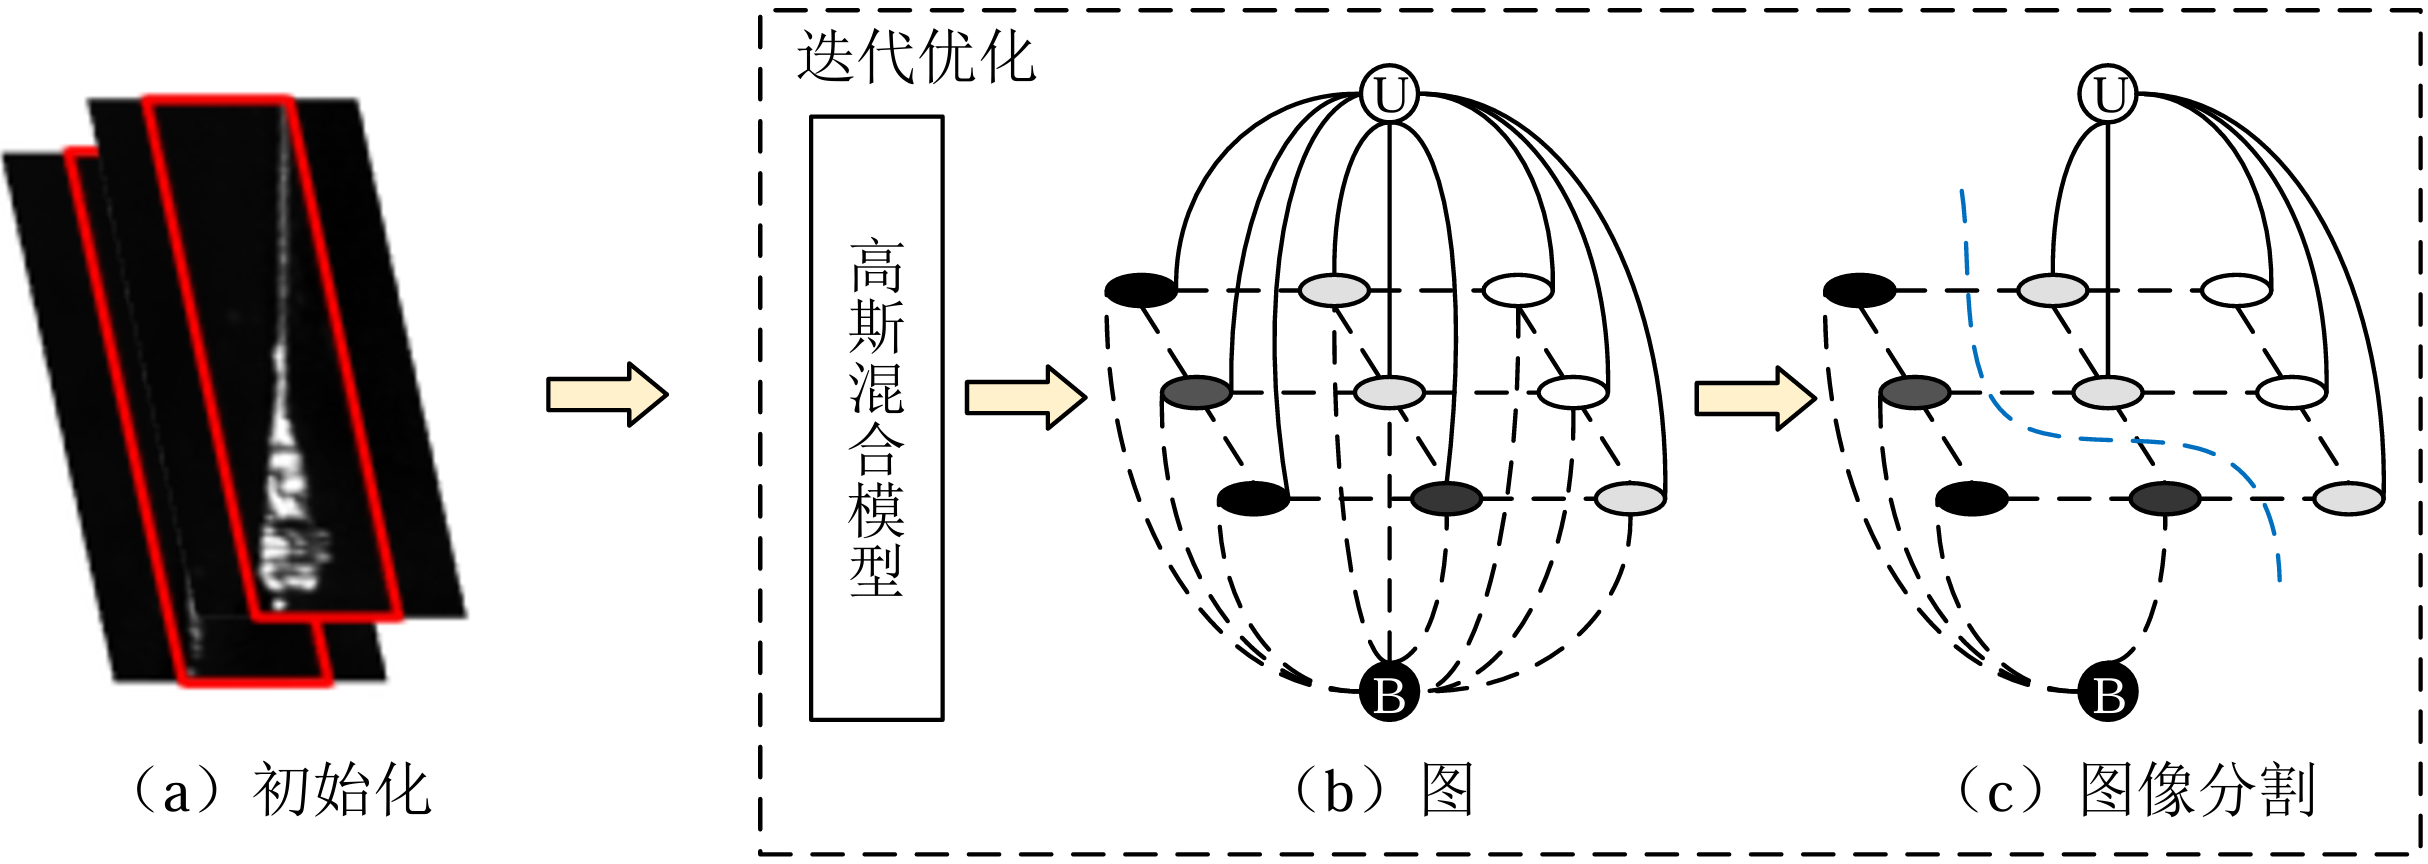
\includegraphics[width=0.95\linewidth]{Figure/GrabCut}
				\caption{基于 GrabCut 模型的刀具磨损区域提取原理}
			\end{figure}
		\end{block}
	\end{frame}

	\begin{frame}
		\begin{block}{GrabCut 分割算法(GMM模型 \& 最小割最大流模型)}
			\qquad 我们自己利用 MATLABR2024a 测试了一下 GrabCut 算法的效果,如下图所示:
			\begin{figure}[H]
				\centering
				\subfloat[测试原图]{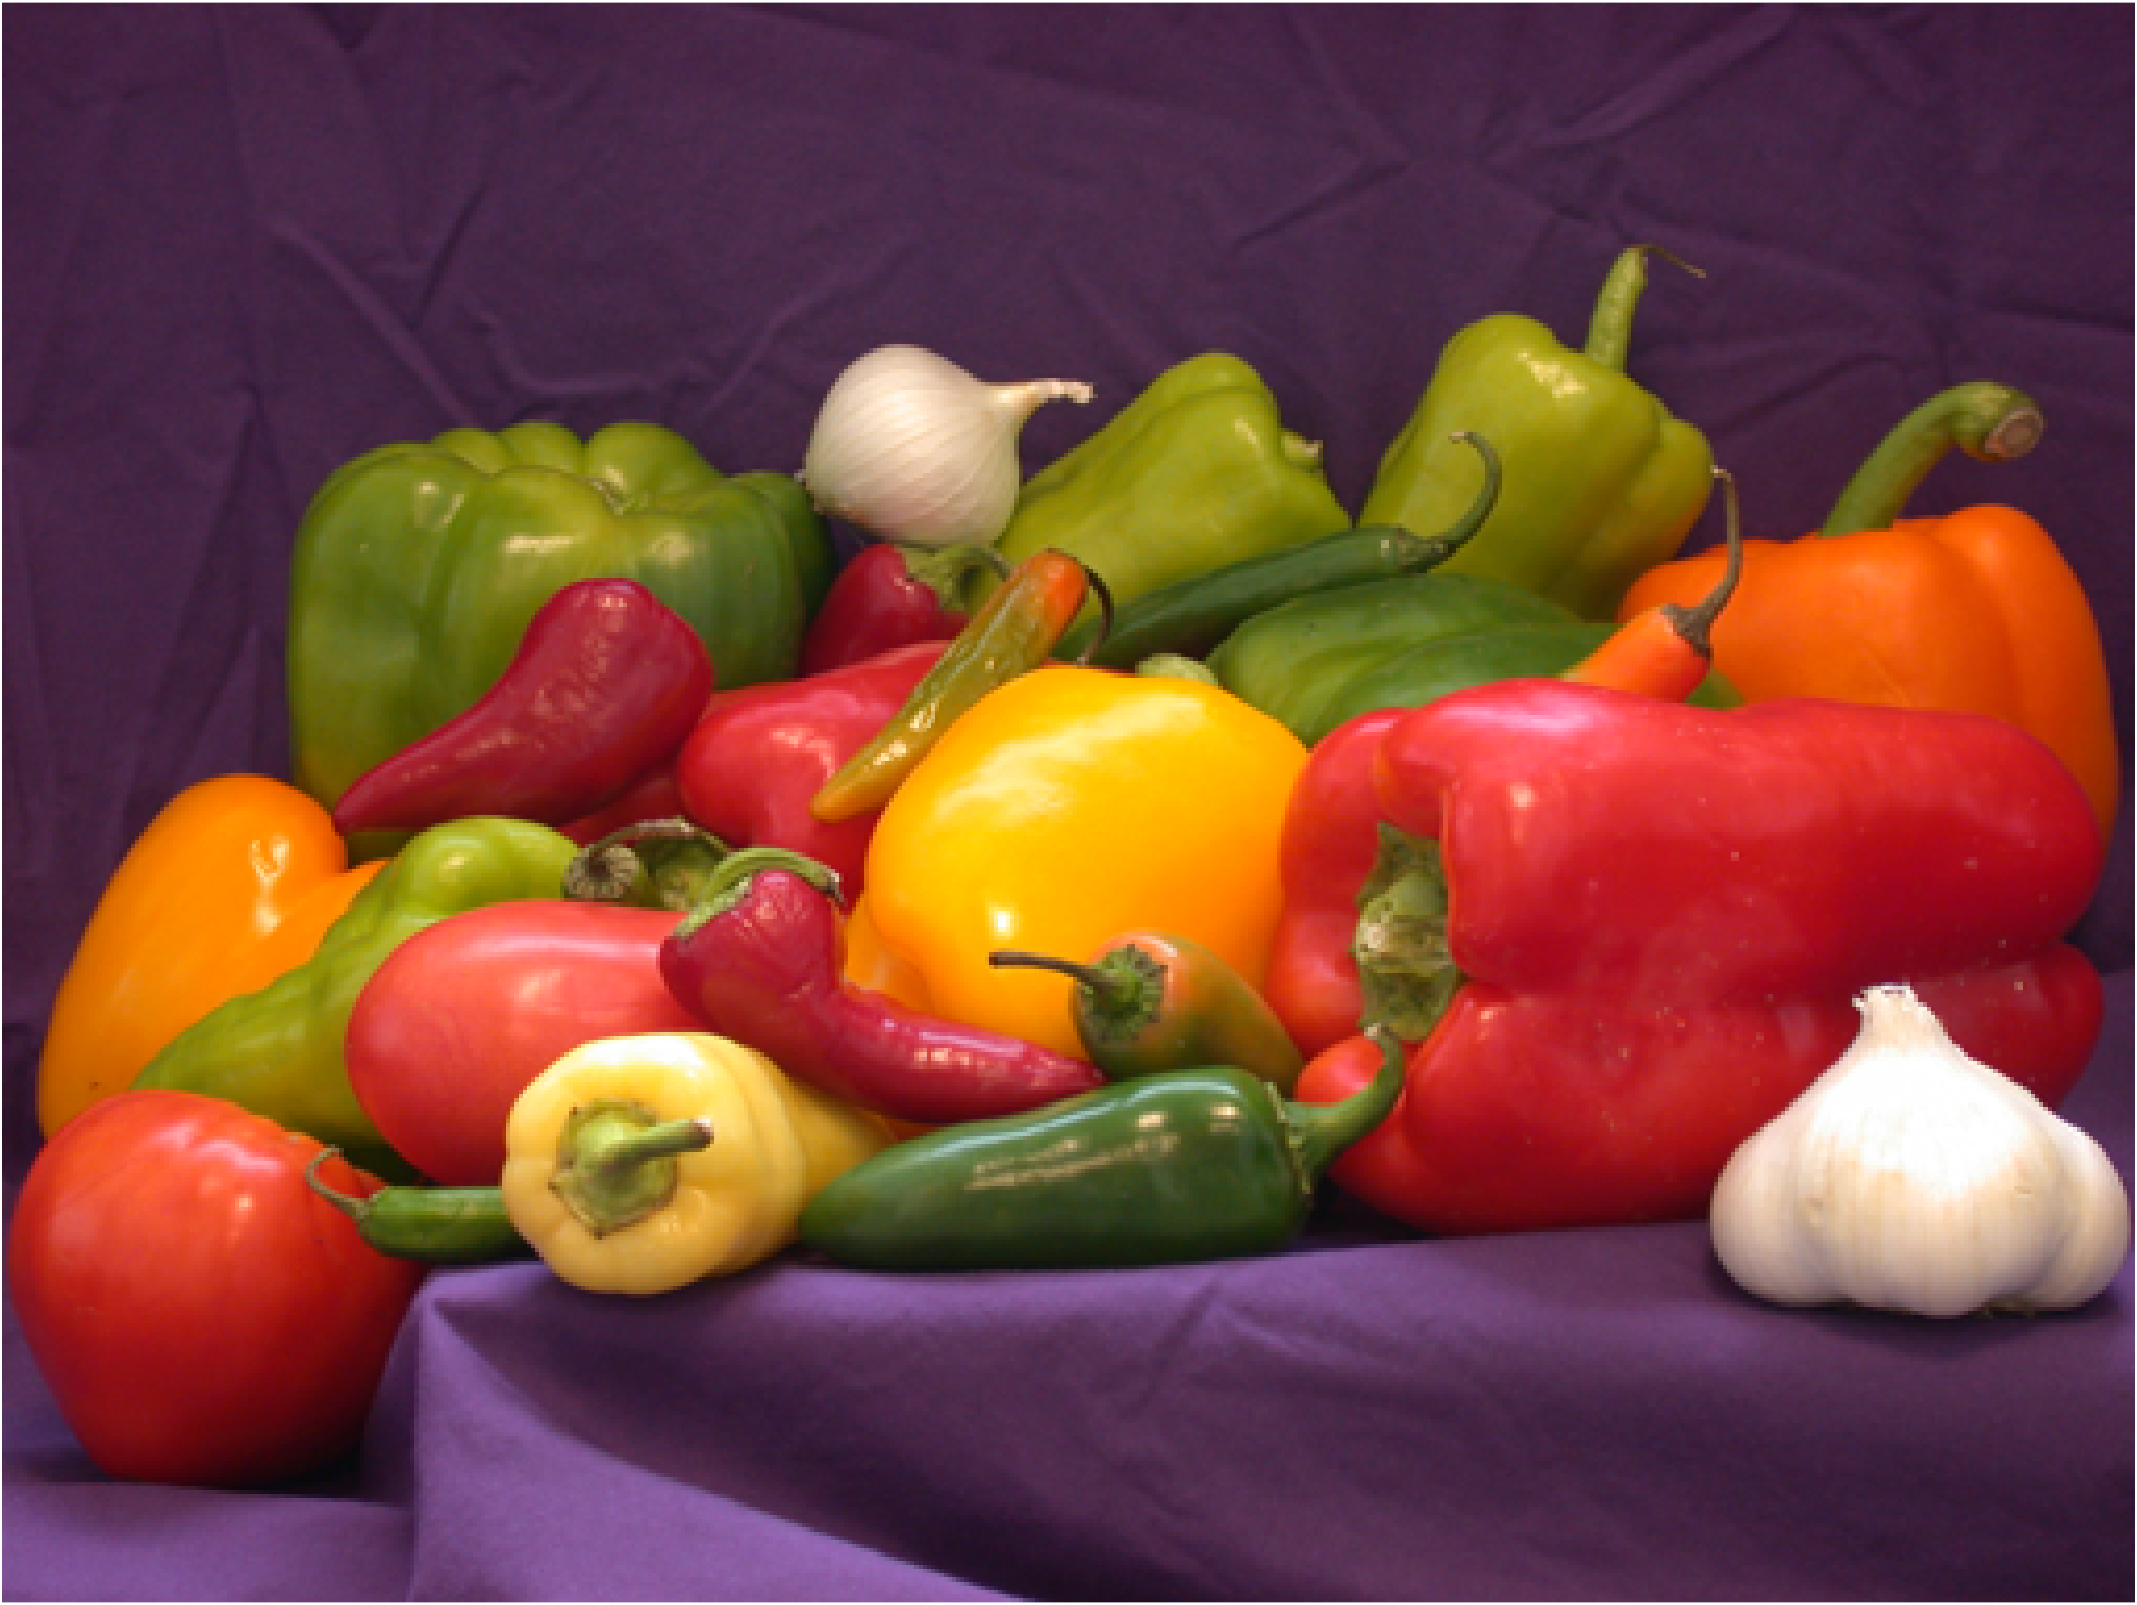
\includegraphics[width=0.45\linewidth]{Figure/test1}}
				\hspace*{12pt}
				\subfloat[测试图分割]{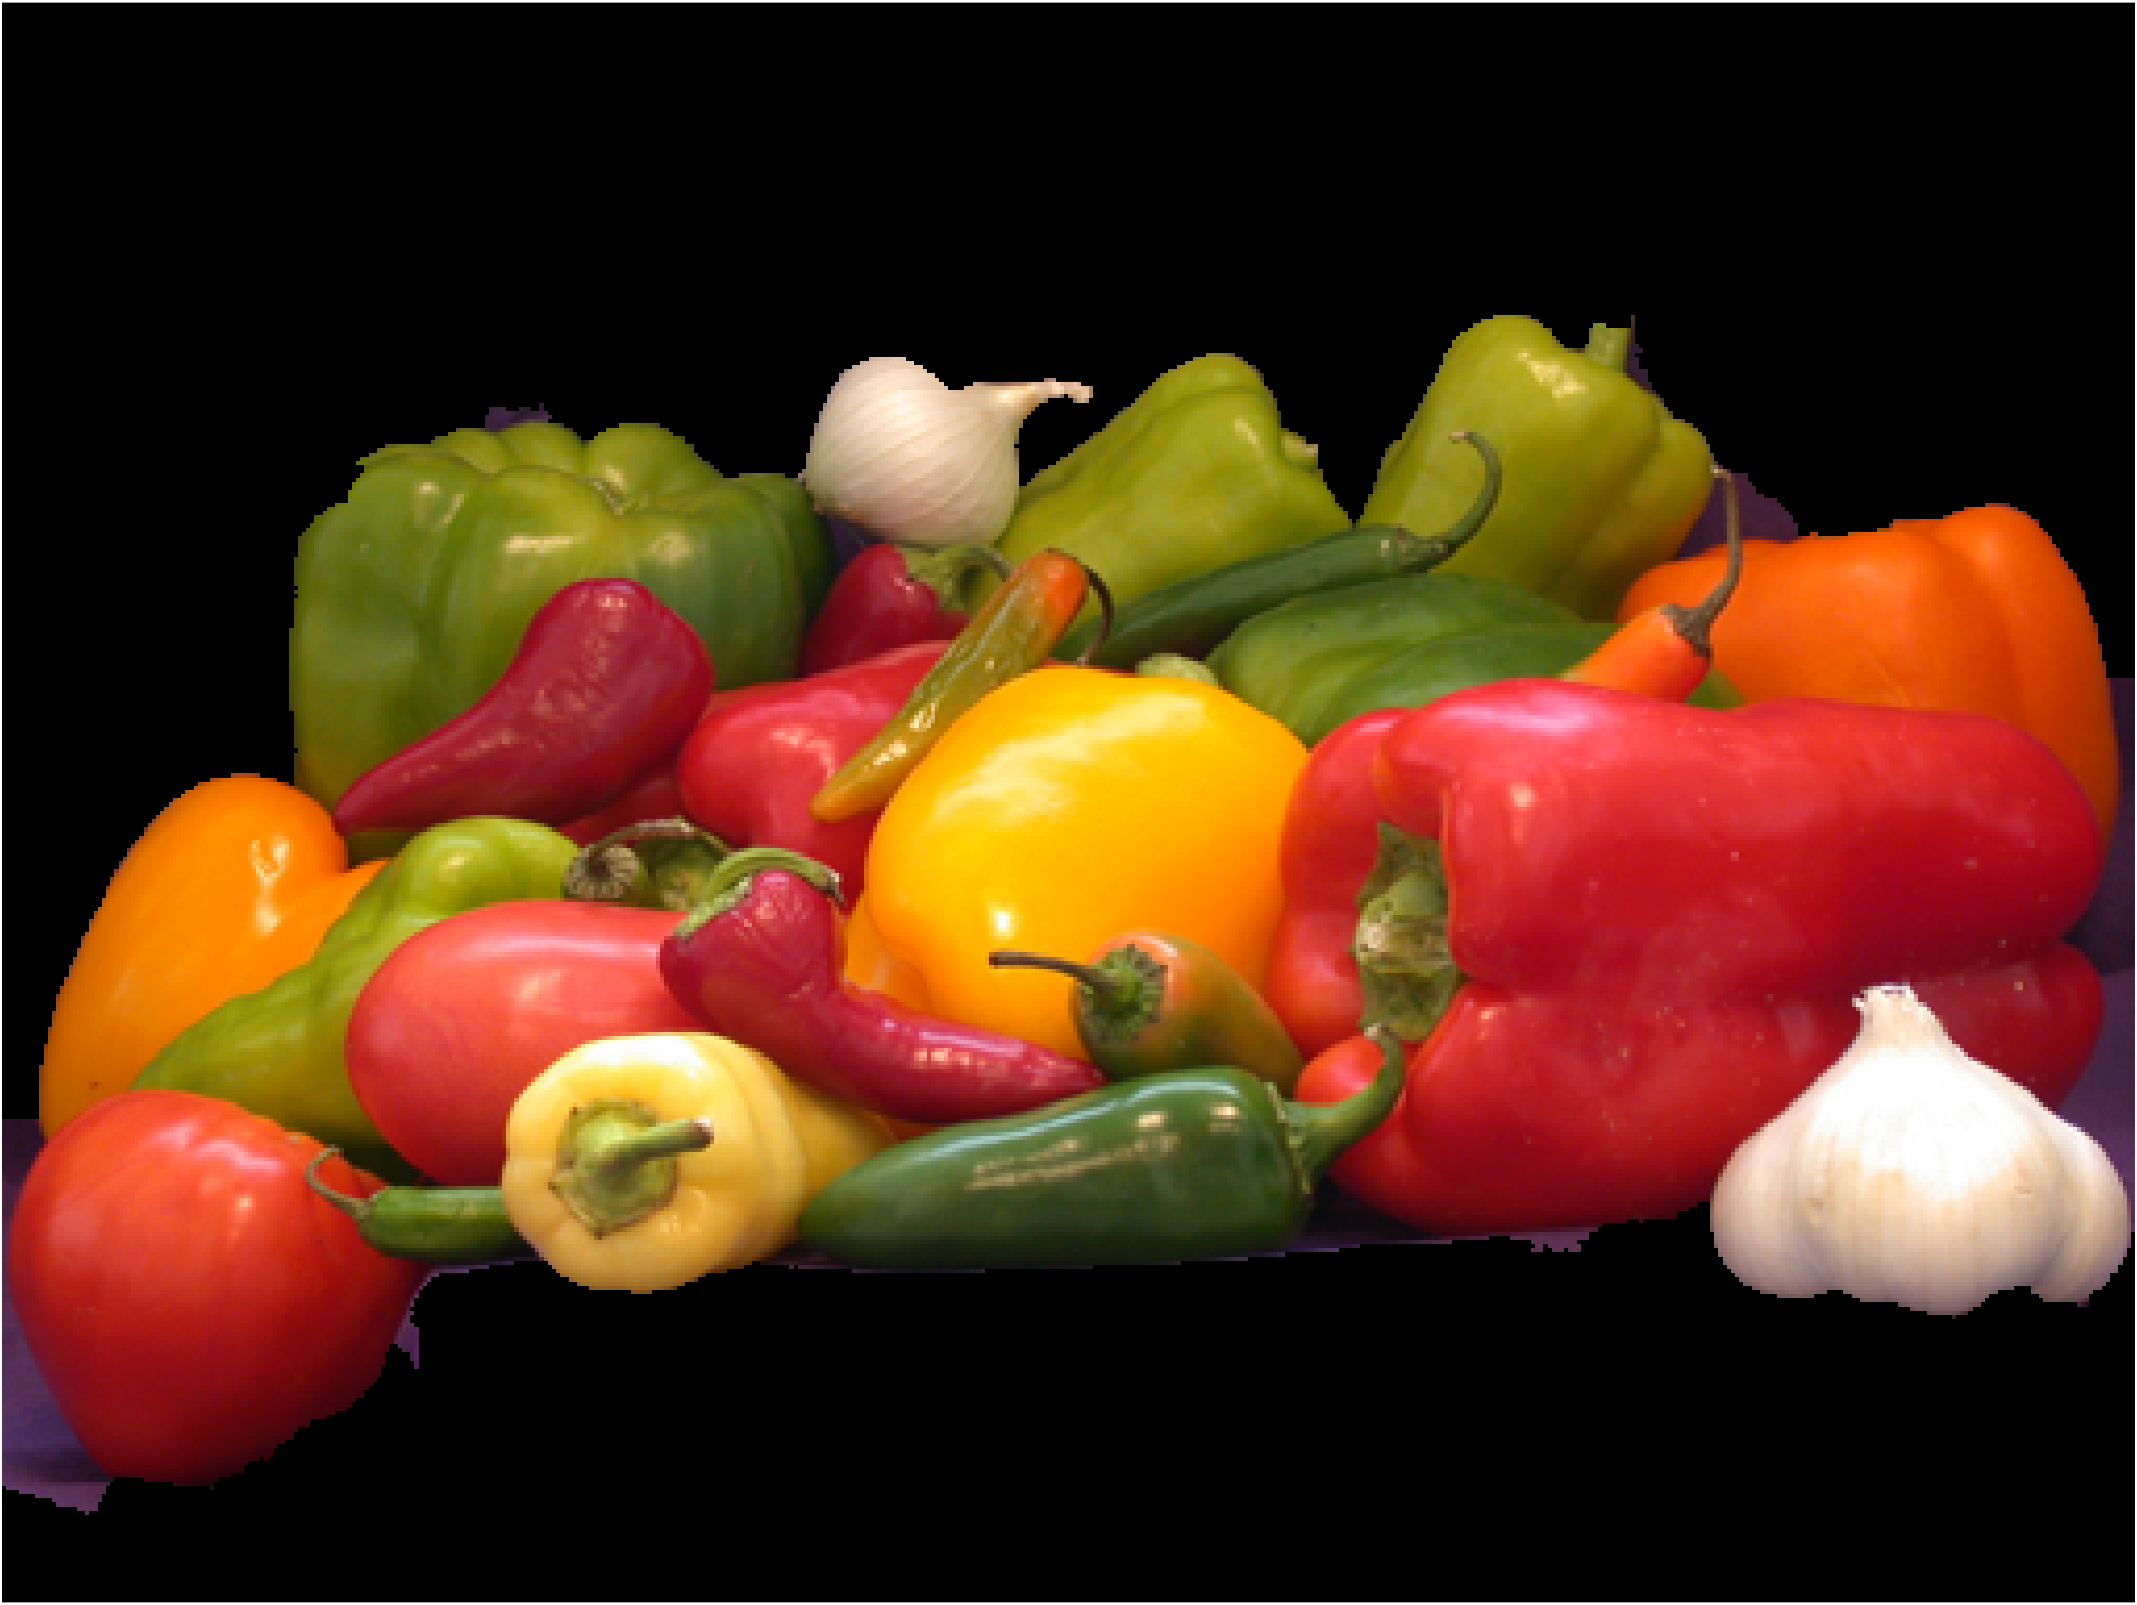
\includegraphics[width=0.45\linewidth]{Figure/test2}}
			\end{figure}
			
			\qquad 可以看出,该算法可以有效地分离前景和背景,大多数市面手机中的消除或者物体提取都有该算法的身影。
		\end{block}
	\end{frame}
	
	\begin{frame}
		\begin{block}{OLS 测量模型}
			\qquad 主切削刃上条带磨损区域如下图所示:
			\begin{figure}[H]
				\centering
				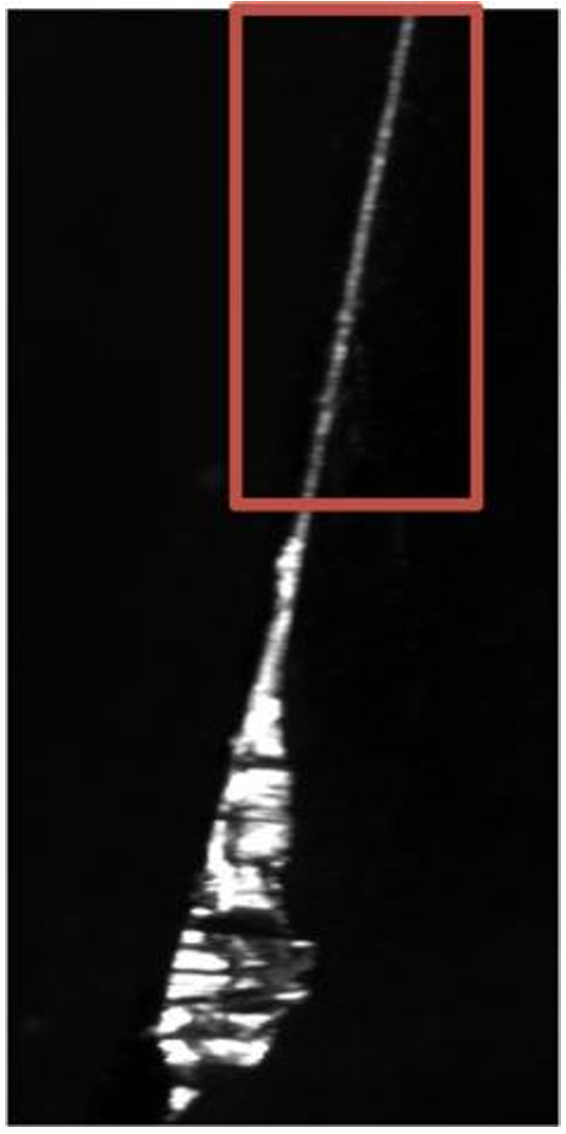
\includegraphics[width=0.15\linewidth]{Figure/mosun}
				\caption{主切削刃上条带磨损区域}
			\end{figure}
			\qquad 包围矩形范围为 $M\times N$,每行磨损区域的中点作为主切刃直线上的点 $(x_i,y_i),i=1,2,\dots,M$。设拟合的主切削刃所在直线为
			\begin{equation}
				y=\alpha x+\beta
				\label{OLS}
			\end{equation}
		\end{block}
	\end{frame}
	
	
	\begin{frame}
		\begin{block}{OLS 测量模型}
			\qquad 利用最小二乘法容易求解 \eqref{OLS} 的拟合问题,这里不再赘述。对于已经求解出的 \eqref{OLS} 模型,利用点到直线距离求得后刀面最大磨损值
			\begin{equation}
				VB = \max\left(\sigma\left|\dfrac{\alpha x_i-y_i+\beta}{\sqrt{1+\alpha^2}}\right|\right)
			\end{equation}
			其中,$(x_i,y_i)$ 是分割出的磨损区域的点像素坐标;$\sigma$ 为像素到真实物理距离的比例。
			
			\qquad 拟合结果如下:
			\begin{figure}[H]
				\centering
				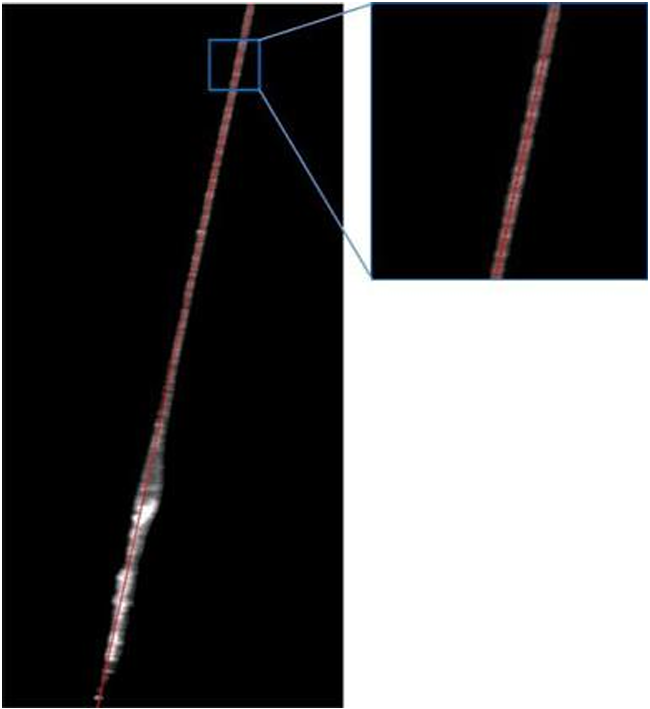
\includegraphics[width=0.3\linewidth]{Figure/Res2}
				\caption{主切削刃上条带磨损区域}
			\end{figure}
		\end{block}
	\end{frame}


	% #################### section4 ####################
	\section{实验设计与结果分析}
	% 每个 section 开始之前,生成当前目录
	\setLayout{mainpoint} % 当前 frame 的布局,可选择:'horizontal','vertical', 'blank, 'mainpoint', 'titlepage'
	\begin{frame}
		\frametitle{实验设计与结果分析}
	\end{frame}

	\setLayout{vertical} % 当前 frame 的布局,可选择:'horizontal','vertical', 'blank, 'mainpoint', 'titlepage'
	\subsection{实验设计}
	\begin{frame}
		\frametitle{实验设计}
		\begin{block}{加速铣刀寿命实验的切削加工参数}
			\qquad 由于面铣刀加工效率高,结构强度高,可以使用较快的进给速度,且加工平面为零件制造中最为常见的加工方式。因此,在本章中,面铣刀被选为待监测对象。其加工参数如下表所示:
			\begin{table}[H]
				\centering
				\caption{BT-2307 双远心镜头参数}
				\begin{tabular}{cc|cc}
					\toprule[1.5pt]
					参数 & 数值 & 参数 & 数值 \\
					\midrule[0.75pt]
					主轴转速(r/min)  & 3000 & 切削速度(mm/min) & 200 \\
					背吃刀量(mm) & 1 & 刀具型号 & Duracarb APMT1135 \\
					工件尺寸(mm) &  $50\times60\times100$ & 工件材料 & 45 钢 \\
					\bottomrule[1.5pt]
				\end{tabular}
			\end{table}
		\end{block}
	\end{frame}
	
	\begin{frame}
		\begin{block}{铣刀监测系统}
			\qquad 铣刀监测系统如下图所示:
			\begin{figure}[H]
				\centering
				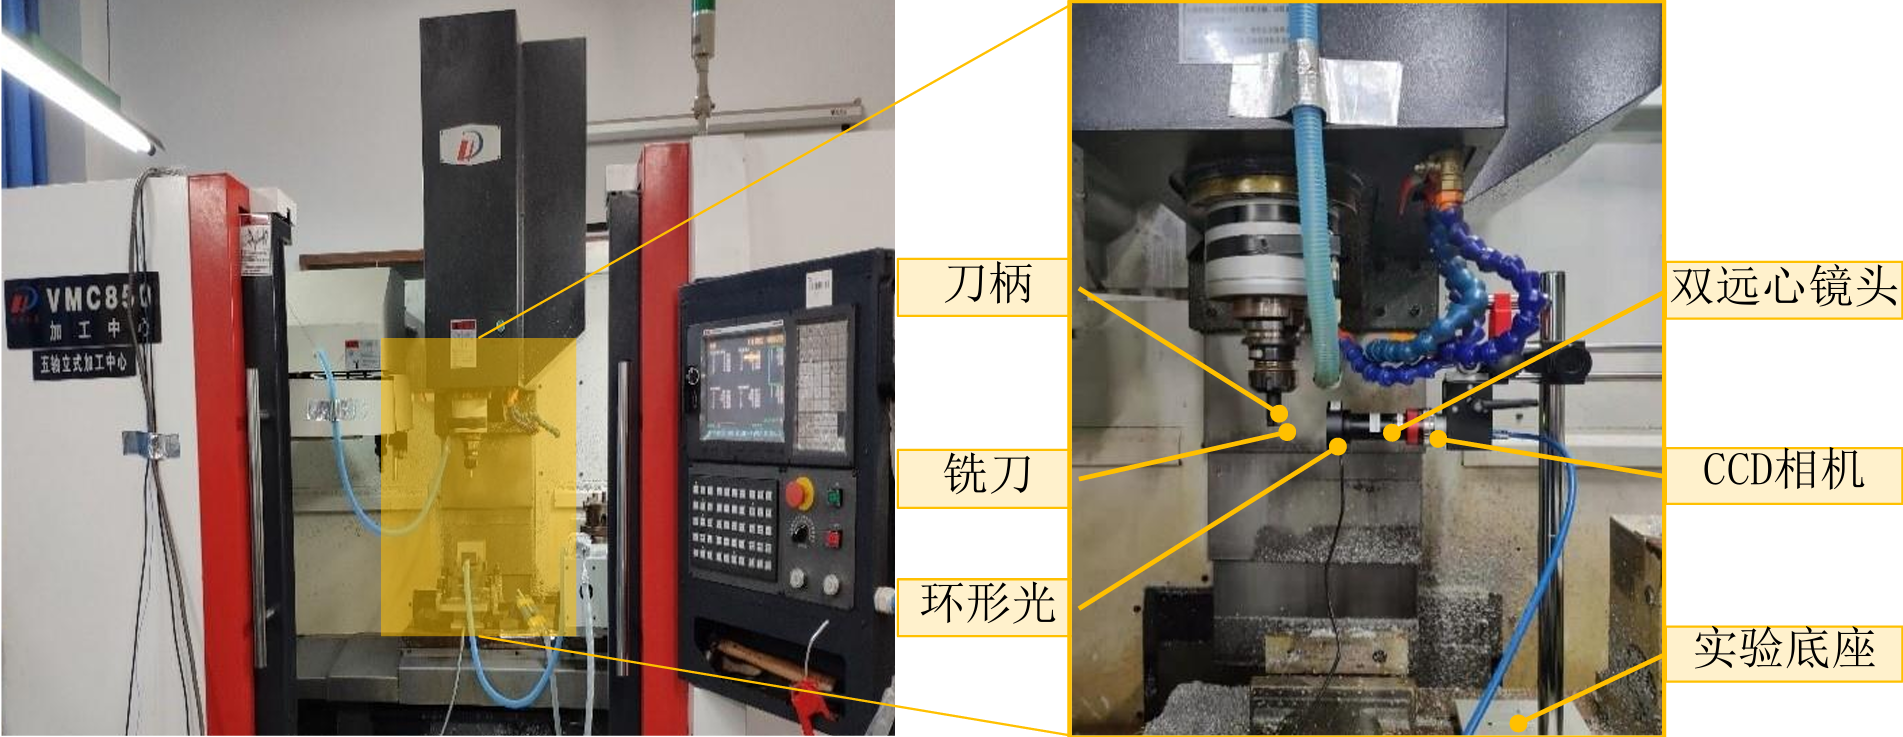
\includegraphics[width=0.8\linewidth]{Figure/shiyanxitong}
				\caption{铣刀监测系统}
			\end{figure}
		
			\qquad 实验中配备了显微镜,将算法结果与显微镜结果比对从而评价测量精度。
		\end{block}
	\end{frame}
	
	\subsection{结果分析}
	\begin{frame}
		\frametitle{结果分析}
		\begin{block}{图像分割结果}
			\qquad 图像分割结果如下图所示:
			\begin{figure}[H]
				\centering
				\subfloat[原始图像]{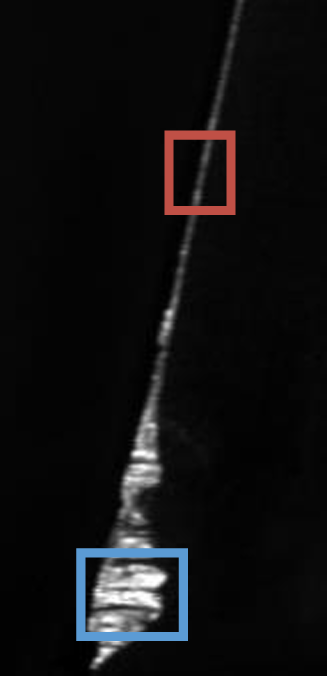
\includegraphics[width=0.16\linewidth]{Figure/yuanshi}}
				\hspace*{24pt}
				\subfloat[提出方法]{
\includegraphics[width=0.16\linewidth]{Figure/tichu}}
				\hspace*{24pt}
				\subfloat[分水岭法]{
\includegraphics[width=0.16\linewidth]{Figure/fenshuiling}}
				\hspace*{24pt}
				\subfloat[OTSU 法]{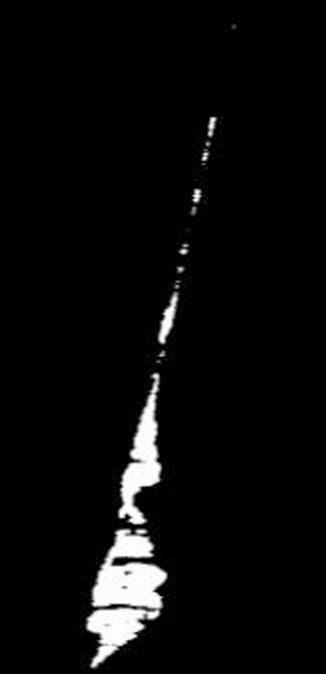
\includegraphics[width=0.16\linewidth]{Figure/OTSU}}
				\caption{图像分割结果}
			\end{figure}
		\end{block}
	\end{frame}

	\begin{frame}
		\begin{block}{磨损测量结果}
			\qquad 磨损测量结果如下图所示:
			\begin{figure}[H]
				\centering
				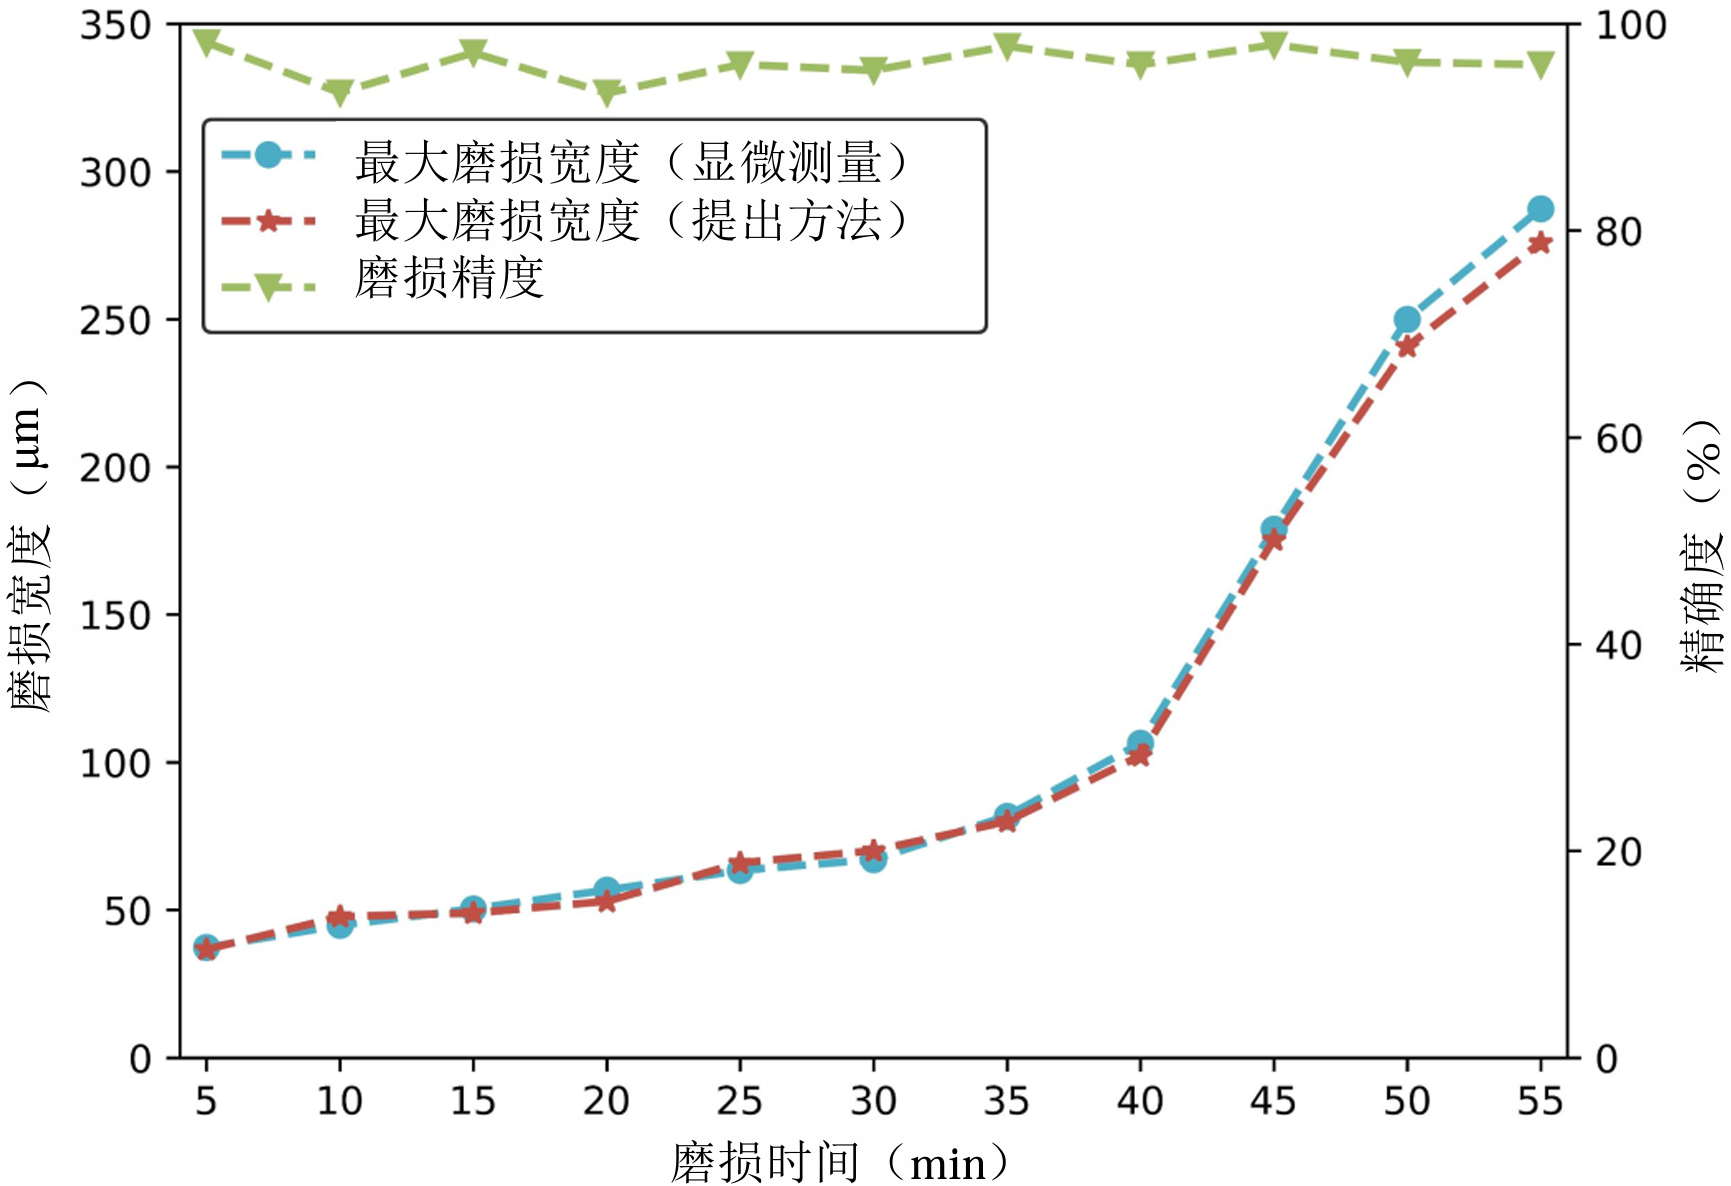
\includegraphics[width=0.55\linewidth]{Figure/Res3}
				\caption{磨损测量结果($\sigma=4.125\mathrm{\mu m}$)}
			\end{figure}
			
			\qquad 提出算法的测量精度在 {\color[RGB]{157,187,101}93.28\%} 到 {\color[RGB]{157,187,101}98.18\%} 范围,这里的精度是{\color[RGB]{193,81,67}提出方法的测量值}除以{\color[RGB]{74,172,197}显微镜的测量值}。例如,在机械加工 8 分钟之后,通过显微镜测量的刀面最大磨损量为 {\color[RGB]{74,172,197}$37.31\mathrm{\mu m}$},同时提出的方法估计的最大磨损量为 {\color[RGB]{193,81,67}$36.63\mathrm{\mu m}$},测量精度高达 {\color[RGB]{157,187,101}98.18\%}。
		\end{block}
	\end{frame}
	
	% #################### 结尾页 ####################	
	\setLayout{titlepage}
	\begin{frame}
		\centering
		\Huge
		\vfill
		感谢观看!
	\end{frame}

\end{document}